\documentclass[../main.tex]{subfiles}

\begin{document}

\section{DIS, nucleon structuur, PDF's}%
\label{sec:dis_nucleon_structuur_pdf_s}

\subsection{Diep inelastische verstrooiing}%
\label{sub:diep_inelastische_verstrooiing}

\begin{figure}[h]
    \centering
    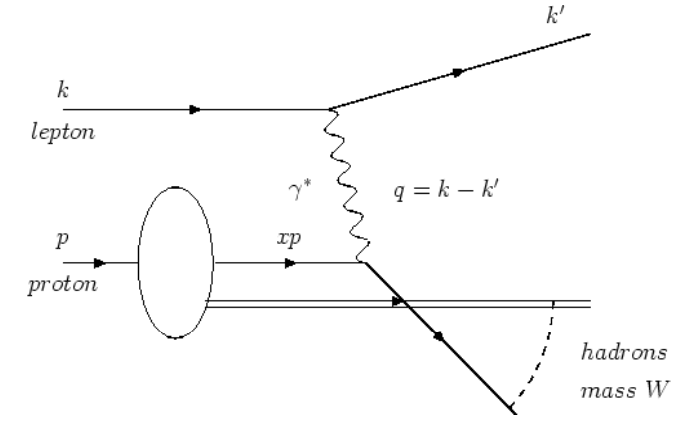
\includegraphics[width=0.8\linewidth]{DIS_nucleon_structuur_pdf/diep_in_ver.png}
    \caption{Diep inelastische verstrooiing van een proton en een lepton}%
    \label{fig:diep_in_ver}
\end{figure}

Bij deze verstrooiing zal de kinetische energie van het lepton veel hoger zijn dan de massa van proton. Zo is het mogelijk om de inwendige structuur van het proton te gaan bekijken. De reden waarom we dit kunnen doen is omdat bij deze hoge energieën de golflengte van het foton veel kleiner zal zijn dan de grote van het proton. In dit geval werken we met een foton wat een groot voordeel is omdat we de vertices in dit diagram heel goed kunnen beschrijven en het lepton is een elementair deeltje. De enige onbekende in dit systeem is dus de inwendige structuur van het proton. De reden waarom het zo lang heeft geduurd voor we proton bundels zijn beginnen gebruiken is omdat niet alle massa in de valentie quarks van het proton zullen zitten wat het allemaal veel ingewikkelder maakt. Om met het LHC nauwkeurige metingen te kunnen uitvoeren moeten we veel meer statistiek (meer events) hebben.\\
De kinetiek van het proces schematisch weergegeven in figuur \ref{fig:diep_in_ver} kan makkelijk neergeschreven worden. Een parton (quark) van een proton met 4moment $xp$ zal een energie $q$ absorberen van het foton en een vrij deeltje worden.
\begin{equation}
    \begin{aligned}
        \label{eq:parton_foton_abs}
        \text{voor absorptie: }(xp+q)^2 &= m_{parton}^2 \approx 0\\
                                        &=x^2p^2+2xpq+q^2\\
                                        &=2xpq+q^2\\
                          \Rightarrow x &=- \frac{-q^2}{2pq} = \frac{Q^2}{2pq} 
    \end{aligned}
\end{equation}
Het enige deeltje dat in staat zal zijn om een foton met energie $q$ te absorberen moet een impulsfractie $x$, zoals berekend in (\ref{eq:parton_foton_abs}), hebben van het proton. Met andere woorden hebben we een filter op welke partonen we willen waarnemen. Deze fractie is Lorentz invariant en dimensieloos. Een andere Lorentz invariante grootheid in dit proces is $y=\frac{q\cdot p}{k\cdot p}$. Deze geeft de fractie van het elektron dat gedragen wordt door het foton.\\
Verder uitgewerkt op een vast target hebben we als 4 momenta:
\begin{equation}
    \begin{aligned}
        \label{eq:4_momenta_dis}
        k=
        \begin{pmatrix}
            E\\
            0\\
            0\\
            E
        \end{pmatrix},
        p=
        \begin{pmatrix}
            m_p\\
            0\\
            0\\
            0
        \end{pmatrix},
        k'=
        \begin{pmatrix}
            E'\\
            0\\
            E'\sin\theta\\
            E'\cos\theta
        \end{pmatrix},
        p_h=
        \begin{pmatrix}
            E_h\\
            p_{xh}\\
            p_{yh}\\
            p_{zh}\\
        \end{pmatrix}
    \end{aligned}
\end{equation}
De aannames dat we hier hebben gedaan zijn:
\begin{itemize}
    \item elektron beweegt langs de z-as
    \item door hoge energieën zien we het elektron als massaloos: $|E_e|=|p_{ze}|$
    \item het elektron verstrooit in het yz-vlak
    \item De hadronische finale toestand is de som van alle uitkomende deeltjes samen
\end{itemize}
De invariante massa van dit systeem is $W=\sqrt{E_H^2-\vec{p}^2_h}\geq m_p$. Het is mogelijk maar zeldzaam dat de geabsorbeerde energie kan verdeeld worden onder alle andere partons om zo een proton uit te komen. Dit is een elastische verstrooiing en $W=m_p$. In alle andere gevallen breekt het parton los van de rest en hebben we een inelastische verstrooiing met $W>m_p$.\\
Dit systeem heeft 8 vrijheidsgraden (voor zowel $k'$ als $p_h$ 1 voor de energie en 3 voor de hoeken). Eén van deze vrijheidsgraden valt weg vanwege de massa van het elektron dat verwaarloosd wordt, nog 4 vallen weg door het behoud van energie en impuls en ten laatste valt er nog 1 weg door azimutale symmetrie. Zo houden we uiteindelijk nog 2 vrijheidsgraden over. De 2 makkelijkst te kiezen variabelen zijn $E'$ en $\theta$. Het probleem hierbij is dat deze niet Lorentz invariant zijn. Deze variabelen kunnen wel omgevormd worden naar $x$ en $y$ die dit wel zijn.
\begin{equation}
    \begin{aligned}
        \label{eq:etheta_naanr_xy}
        \begin{matrix}
            Q^2 & = & -(k-k')^2                 & \approx   & 2EE'(1-\cos\theta) \\
            x   & = & -\frac{q^2}{2p\cdot q}    & =         & \frac{EE'(1-\cos\theta)}{(E-E')m_p} \\
            y   & = & -\frac{q\cdot p}{k\cdot p}& =         & \frac{E-E'}{E} \\
        \end{matrix}
    \end{aligned}
\end{equation}

\subsection{Experimenten}%
\label{sub:experimenten}

\begin{figure}[h]
    \centering
    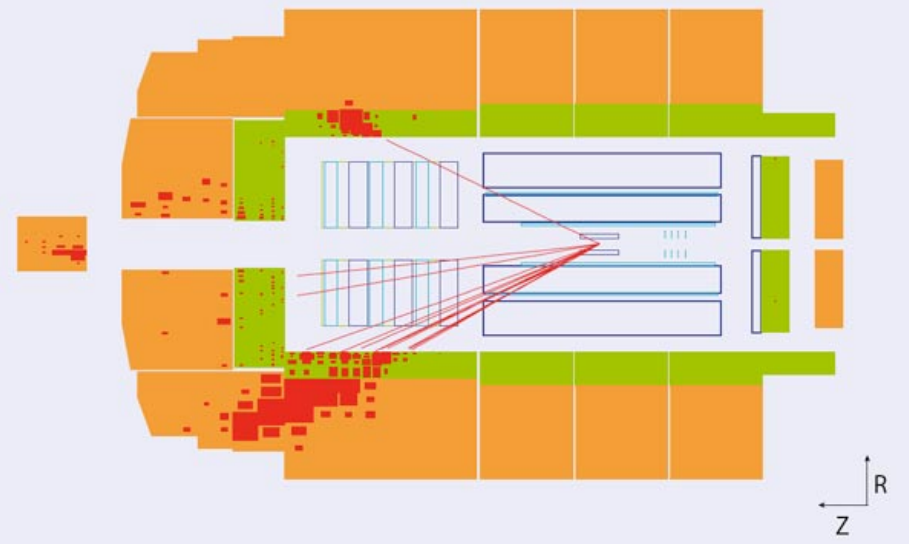
\includegraphics[width=0.6\linewidth]{DIS_nucleon_structuur_pdf/hera.png}
    \caption{HERA experiment}%
    \label{fig:hera}
\end{figure}

De beste vaste target machines voor precisie zijn $e^+e^-$ colliders. Op deze machines zijn ook voor het eerst de quarks gezien. In het CERN hadden ze eerst een proton collider gemaakt en dachten dat ze de boot gemist hebben. Wat ze gedaan hebben is de protonen op een target insturen en daar komen massa's pionen uit. Als je deze lang genoeg meeneemt, gaan die vervallen naar muonen met een levensduur van de orde $10^{-8}$s en zo verkrijgen we een muon bundel. Omdat dit tertiaire deeltjes zijn gaat de densiteit van de deeltjes veel lager liggen en zullen een vrij breed energiespectrum hebben. Hetzelfde kan gedaan worden voor neutrino's.\\
Er zijn ook colliders waar 2 deeltjes bundels op elkaar worden afgestuurd. Een voorbeeld van de waargenomen deeltjes is in figuur \ref{fig:hera} gegeven van het HERA experiment. Hier is het duidelijk dat de elektronen van links zullen komen. Dit omdat de inkomende energie van het proton veel hoger is dan dat van het elektron en de uitgaande deeltjes van de collisie gaan wegens behoud van impuls via de linker kant de detector verlaten.\\
Als je zo een extravagant experiment zoals het LHC maakt is 1 van de eerste dingen die je doet het onderzoeken van het  kinematisch bereik van dat experiment. In figuur \ref{fig:kin_bereik} wordt $Q^2$ in functie van $x$ geplot van verschillend colliders.

\begin{figure}[h]
    \centering
    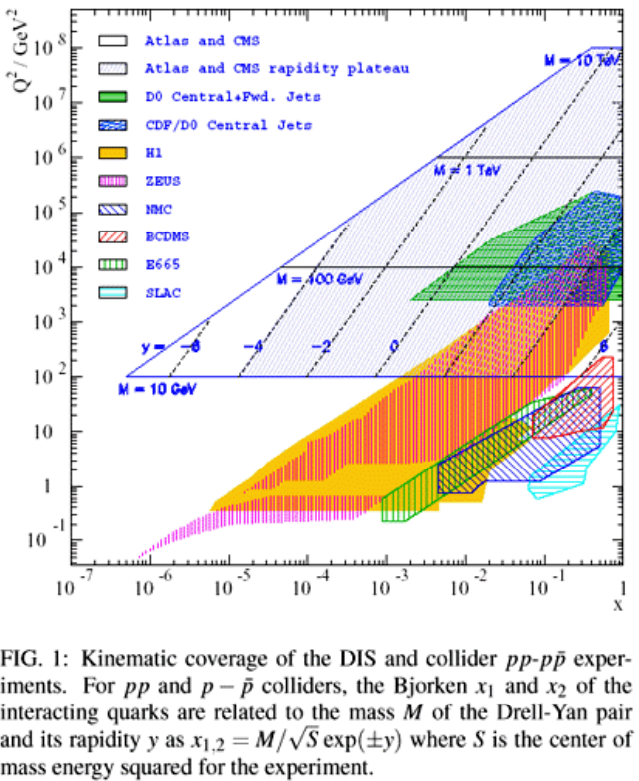
\includegraphics[width=0.8\linewidth]{DIS_nucleon_structuur_pdf/kin_bereik.png}
    \caption{Kinematisch bereik}%
    \label{fig:kin_bereik}
\end{figure}

\subsection{Cross section}%
\label{sub:cross_section}

De werkzame doorsnede van deze DIS experimenten wordt gegeven door:
\begin{equation}
    \begin{aligned}
        \label{eq:dis_werkzame_doorsnede}
        \frac{d^2\sigma^{e,N}}{dxdy} = \frac{4\pi\alpha^2s}{Q^4} [xy^2F_1^{eN}+(1-y)F_2^{eN}]
    \end{aligned}
\end{equation}
met $F_1$ en $F_2$ de structuur functies. Het is logisch dat er in deze werkzame doorsnede een $\alpha^2$ afhankelijkheid verwerkt zit omdat deze interactie verloopt via de elektromagnetische interactie en dus 2 vertices heeft die elk een $\alpha$ toedragen. En de waarschijnlijkheid dat we de impulsfractie $x$ vinden van het parton wordt gegeven door die structuur functies $F_1$ en $F_2$. Het zijn deze dus die alle informatie bevatten. We zien dat de structuur functies afhangen van zowel $x$ als $Q^2$, $F_i(x, Q^2)$. Zo weten we direct dat dit geen puntdeeltjes kunnen zijn omdat we anders geen afhankelijkheid zouden hebben van $Q^2$.\\
{\color{blue}Intermezzo: waar komt de massa van het proton nu vandaan? De structuur van protonen bestaat uit quarks en gluonen. In het echt is dit nog veel complexer dan zomaar die 3 quarks. De uiteindelijke reden daarvoor is dat het proton zeer klein is omdat de interactie tussen quarks zeer sterk is. De quarks worden op ongeveer 1fm van elkaar af. Het heisenberg principe zegt dat als we iets opsluiten in een ruimte van 1fm dat het een nulpuntsenergie van 197MeV zal hebben. De bewegingsenergie/bindingsenergie van de 3 quarks samen is 600MeV. Het grootste gedeelte van de massa van het proton zal dus afhangen van de bewegings-/bindingsenergie van de quarks en niet van de quarks zelf. Deze bindingsenergie komt van de interactie tussen de quarks zelf aan de hand van uitwisseling van gluonen. Door het continu uitgewisselde gluonen splitsen continu in quark-antiquark paren. Dit is het equivalent van de lamb shift in elektronenwolken.}\\
Het is nog nooit gelukt om de structuur functies wiskundig uit te rekenen, QCD is hier niet toe in staat. De enige manier om deze te bepalen is aan de hand van experimenten. In het quark parton model kunnen we $F_2$ uitschrijven
\begin{equation}
    \begin{aligned}
        \label{eq:tweede_structuur_functie}
        F_2^{eN}(x)=\sum_q xQ_q^2|q^N(x)+\overline q^N (x)]
    \end{aligned}
\end{equation}
Hier sommeren we over alle quarks. $q^N(x)$ en $\overline q^N(x)$ zijn respectievelijk de waarschijnlijk om een quark of antiquark in het proton te vinden. Al dat we hier alle mogelijke quarks bekijken is het zo goed als onmogelijk een top quark met een massa van $\pm100$GeV tegen te komen in een proton van 1GeV. Er is een relatie tussen $F_1$ en $F_2$
\begin{equation}
    \begin{aligned}
        \label{eq:struct_func_rel}
        \frac{2xF_1}{F_2} =
        \begin{matrix}
            1 & & \text{spin } \frac{1}{2} \\
            0 & & \text{spin } 0
        \end{matrix}
    \end{aligned}
\end{equation}
Deze relatie is makkelijk aangetoond.
\begin{equation}
    \begin{aligned}
        \label{eq:bewijs_struct_func_rel_1}
        \left(\frac{d\sigma}{d\Omega}\right)_{puntdeeltje,1/2)} = {\color{red} \left(\frac{d\sigma}{d\Omega}\right)_{Rutherford}\cos^2  \frac{\theta}{2}} {\color{green} \left[1+ \frac{2Q^2}{4m^2c^2} \tan^2 \frac{\theta}{2} \right]}
    \end{aligned}
\end{equation}
n het rood vinden we de Mott cross sectie $\left(\frac{d\sigma}{d\Omega}\right)_{M}$, de cross sectie voor het verstrooien van een spin $1/2$ deeltje aan een spin $0$ deeltje. Uit de Rutherford cross sectie komt uiteindelijk $\alpha^2/Q^4$. De $\cos^2$ in de Mott cross sectie komt uit het behoud van heliciteit en angulair moment. Als je een elekton hebt met spin 1/2 dan is zijn heliciteit de projectie van zijn spin op de bewegingsrichting. In het geval dat we een positieve heliciteit hebben liggen de bewegingsrichting en heliciteit in dezelfde richting. Onder een verstrooiing van $180^\circ$ zal de spin van het deeltje niet verandert zijn maar het momentum wel. Dit zorgt ervoor dat de heliciteit en momentum antiparallel zijn wat wegens behoud van heliciteit niet kan. Dit wordt weergegeven in deze cos-term.

\begin{figure}[h]
    \centering
    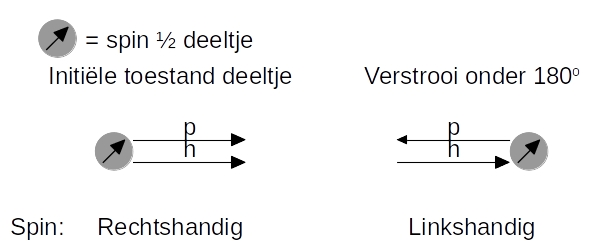
\includegraphics[width=0.8\linewidth]{DIS_nucleon_structuur_pdf/mot_cross_section.jpg}
    \caption{Visualisatie van spin $1/2$ deeltje dat verstrooit onder een hoek van $180^\circ$}%
    \label{fig:mot_cross_section}
\end{figure}

Het toevoegen van het groen gedeelte aan de Mott cross sectie is nodig als we verstrooien van een spin $1/2$ deeltje aan een spin $1/2$ deeltje. De eerste term in het groene gedeelte is afkomstig van de elektrische interactie en de tweede term van de magnetische interactie m.a.w. van de spin. Door deze term is het terug mogelijk om te verstrooien onder $180^\circ$. Voor het verstrooien van een elektron aan een quark moet aan vergelijking (\ref{eq:bewijs_struct_func_rel_1}) nog de lading van het quark $Q_a^2$ vermenigvuldigd worden. De laatste stap is nu de cross sectie op te stellen van een spin $1/2$ deeltje dat zich verstrooit van een proton.
\begin{equation}
    \begin{aligned}
        \label{eq:bewijs_struct_func_rel_2}
        \left(\frac{d\sigma}{d\Omega dE'}\right) = {\color{green} \left(\frac{d\sigma}{d\Omega}\right)_{M} \sum_q Q_q^2 [1+ \frac{Q^2}{4m^2c^2} \tan^2 \frac{\theta}{2}]} {\color{red}q(x)} \frac{{\color{red}dx}}{dE'} 
    \end{aligned}
\end{equation}
Dit komt neer op de waarschijnlijkheid om te verstrooien naar een quark in het groen en de waarschijnlijkheid om een quark te vinden in het rood. Nu kunnen we ad-hoc een aantal dingen uitwerken:
\begin{equation}
    \begin{aligned}
        \label{eq:bewijs_struct_func_rel_3}
        \begin{matrix}
            x = \frac{Q^2}{2M\nu}; & \nu = E-E' & \Rightarrow & \frac{dx}{dE'} = \frac{x}{\nu} 
        \end{matrix}
    \end{aligned}
\end{equation}
en de massa van het de quark is gegeven door $m_q = xM_p$. Vullen we deze in vergelijking (\ref{eq:bewijs_struct_func_rel_2}) in.
\begin{equation}
    \begin{aligned}
        \label{eq:bewijs_struct_func_rel_4}
        \left(\frac{d\sigma}{d\Omega dE'}\right) &= \left(\frac{d\sigma}{d\Omega}\right)_{M} \sum_q Q_q^2 [1+ \frac{Q^2}{4x^2M_p^2c^2} \tan^2 \frac{\theta}{2}]q(x) \frac{x}{\nu}\\
                                                 &\Downarrow\\
        \left(\frac{d\sigma}{d\Omega dE'}\right) &= \left(\frac{d\sigma}{d\Omega}\right)_{M} \left[ \frac{1}{\nu} F_2 + \frac{2}{M^2c^2} \tan^2 \frac{\theta}{2} \right]
    \end{aligned}
\end{equation}
Zo komen op de afgeleides na vergelijking (\ref{eq:dis_werkzame_doorsnede}) en vergelijking (\ref{eq:bewijs_struct_func_rel_4}) overeen. Als $\theta=0^\circ$ dan hebben we enkel $F_2$ en als $\theta=180^\circ$ dan hebben we enkel $F_1$. Specifiek voor $1/2$ partons kunnen we vergelijking (\ref{eq:dis_werkzame_doorsnede}) herschrijven als volgt:
\begin{equation}
    \begin{aligned}
        \label{eq:struct_func_parton}
        \frac{d^2\sigma^{e,N}}{dxdy} &= \frac{4\pi\alpha^2s}{Q^4} \left[y^2 \frac{F_2^{e,N}}{2} + (1-y)F_2^{e,N}\right]\\
                                     &= \frac{4\pi\alpha^2s}{Q^4} \left[\frac{1+(1-y)^2}{2}\right]F_2^{e,N}\\
    \end{aligned}
\end{equation}

\subsection{Structuur functies}%
\label{sub:structuur_functies}

Vervolgens kunnen we kijken hoe de structuur functie er uit ziet van het proton.
\begin{equation}
    \begin{aligned}
        \label{eq:struct_func_proton}
        F_2^{e,p} = x\left(Q_u^2(u+\overline u) + Q_d^2(d+\overline d + s + \overline s)\right)
    \end{aligned}
\end{equation}
Hier worden enkel de waarschijnlijkheden van de up, down en strange (anti)quarks in acht genomen omdat de overige zo goed als niet mogelijk zijn. Het proton en neutron zijn voor de sterke wisselwerking hetzelfde alleen dat een up quark verandert in een downquark. Dit geeft de isospin invarianties
\begin{equation}
    \begin{aligned}
        \label{eq:isospin_invariantie}
        \begin{matrix}
            u(x) \equiv u^p(x) = d^n(x) &   & \overline u(x) \equiv \overline u^p(x) = \overline d^n(x) \\
            d(x) \equiv d^p(x) = u^n(x) &   & \overline d(x) \equiv \overline d^p(x) = \overline u^n(x) \\
            s(x) \equiv s^p(x) = s^n(x) & = & \overline s^p(x) = \overline s^n(x)                       \\
        \end{matrix}
    \end{aligned}
\end{equation}
Gebruiken we deze invariantie dan vinden we direct de structuur functie voor het neutron.
\begin{equation}
    \begin{aligned}
        \label{eq:struct_func_neutron}
        F_2^{e,n} = x\left(Q_d^2(u+\overline u + s + \overline s) + Q_u^2(d+\overline d)\right)
    \end{aligned}
\end{equation}
Om de structuur functie van een nucleon te bepalen middelen we uit over de 2 structuurfuncties.
\begin{equation}
    \begin{aligned}
        \label{eq:struct_func_nucleon}
        F_2^{e,N} &\equiv \frac{F_2^{e,p}+F_2^{e,n}}{2}\\
                  &= \frac{x}{2} \left((Q_u^2+Q_d^2)(u+\overline u + d + \overline d) + 2Q_d^2(s+\overline s)\right)\\
                  &\approx \frac{x}{2} \left( \frac{5}{9} (u+\overline u + d + \overline d)\right)
    \end{aligned}
\end{equation}

\subsection{(Anti)neutrino verstrooiing}%
\label{sub:_anti_neutrino_verstrooiing}

\begin{figure}[h]
    \centering
    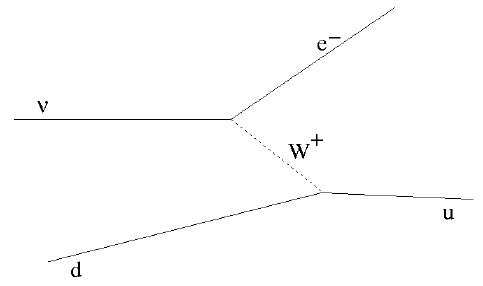
\includegraphics[width=0.8\linewidth]{DIS_nucleon_structuur_pdf/neutrino_scat.png}
    \caption{Feynman diagram van de neutrino verstrooiing}%
    \label{fig:neutrino_scat}
\end{figure}

In principe is het mogelijk voor zowel charged ($W^\pm$) of neutral ($Z^0$) current verstrooiing doen. Hierbij wordt een neutrino afgeschoten op een proton waar na interactie van de neutrino en het quark aan de hand van een W boson het geladen equivalent van de neutrino de verstrooiing verlaten. De neutrino of antineutrino zal door het uitwisselen van respectievelijk ofwel het $W^+$ of $W^-$ boson enkel met een aantal quarks kunnen interageren in het proton:
\begin{itemize}
    \item $\nu$-scattering: $d,\overline u,s$
    \item $\overline \nu$-scattering: $u,\overline d,\overline s$
\end{itemize}
In een experiment kunnen de verschillende (anti)neutrino verstrooiingen uit elkaar gehouden worden omdat $\nu \rightarrow e^-$ en $\overline \nu \rightarrow e^+$. Naast de $F_2^{\nu,N}\propto x(q+\overline q)$ krijgen we nu nog een extra structuur functie $xF_3^{\nu,N}\propto x(q-\overline q)$.
\begin{equation}
    \begin{aligned}
        \label{eq:struct_func_nucleon_zwak}
        \frac{d^2 \sigma^\nu}{dxdy} = \frac{G_F^2 s}{2\pi} \left[ \frac{F_2^\nu+xF_3^\nu}{2} + \frac{F_2^\nu-xF_3^\nu}{2}(1-y^2) \right]
    \end{aligned}
\end{equation}
De eerste term tussen de haakjes zijn enkel de quarks en is onafhankelijk van de hoek waaronder wordt verstrooit en is isotroop. De tweede term zijn de antiquarks is de waarschijnlijkheid om er te hebben afhankelijk van de hoek waaronder verstrooit wordt. Waarom dit zo is wordt snel duidelijk als we de verstrooiing bij $180^\circ$ graden bekijken. Hier hebben we gebruik gemaakt van het feit dat de zwakke wisselwerking enkel bind aan linkshandige deeltjes.

\begin{figure}[h]
    \centering
    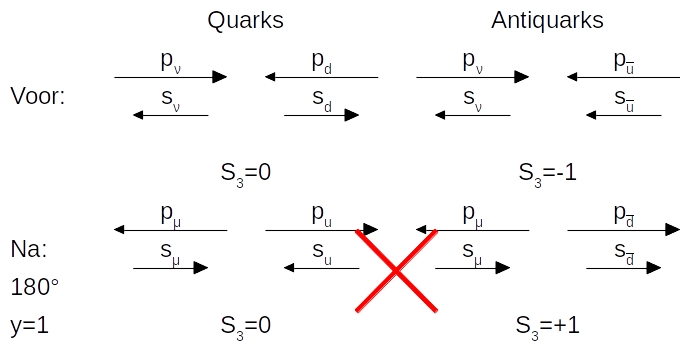
\includegraphics[width=0.8\linewidth]{DIS_nucleon_structuur_pdf/neutr_scat_f_3.jpg}
    \caption{Neurtrino verstrooiing bij $180^\circ$}%
    \label{fig:neutr_scat_f_3}
\end{figure}

Dezelfde redenering kan gedaan worden voor de antineutrinos en dan krijgen we:
\begin{equation}
    \begin{aligned}
        \label{eq:struct_func_nucleon_zwak_anti}
        \frac{d^2 \sigma^{\overline \nu}}{dxdy} = \frac{G_F^2 s}{2\pi} \left[ \frac{F_2^\nu-xF_3^\nu}{2} + \frac{F_2^\nu+xF_3^\nu}{2}(1-y^2) \right]
    \end{aligned}
\end{equation}
Gebruiken we dit nu om de structuurfuncties van het proton en neutron op te stellen.
\begin{equation}
    \begin{aligned}
        \label{eq:struct_func_neutrino_proton_neutron}
        F_2^{\nu, p} &= 2x[d(x)+\overline u(x)]\\
        xF_3^{\nu, p} &= 2x[d(x)-\overline u(x)]\\
        F_2^{\nu, n} &= 2x[u(x)+\overline d(x)]\\
        xF_3^{\nu, n} &= 2x[u(x)-\overline d(x)]\\
                      &\Downarrow\\
        F_2^{\nu, N} &= F_2^{\overline \nu, N}\\
        xF_3^{\nu, N} &= xF_3^{\overline \nu, N}\\
        F_2^{\nu, N} &= x(u+\overline u+d+\overline d)\\
        xF_3^{\nu, N} &= x(u-\overline u+d-\overline d)\\
    \end{aligned}
\end{equation}
Het interessante is dat $xF_3^{\nu, N}$ ons het aantal quarks - het aantal antiquarks geeft m.a.w. de valentie quarks. Experimentezl hebben we kunnen zien dat $F_2$ zowel voor de elektromagnetische als de zwakke wisselwerking hetzelfde is. Dit is het beste bewijs dat we hebben voor de lading van een quark.

\begin{figure}[h]
    \centering
    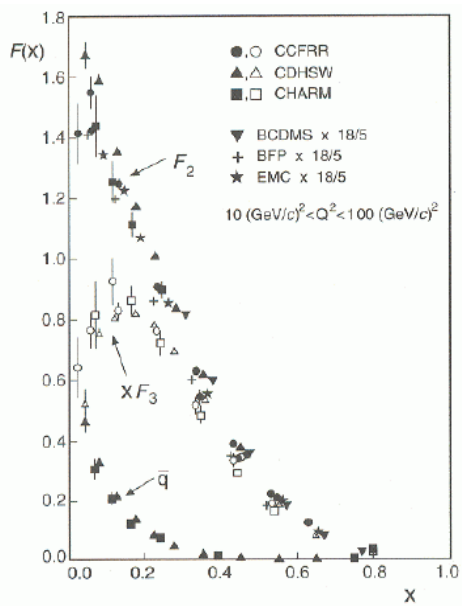
\includegraphics[width=0.4\linewidth]{DIS_nucleon_structuur_pdf/neutr_scat_exp.png}
    \caption{Vergelijking zwakke en EM structuurfunctie in experimenten}%
    \label{fig:neutr_scat_exp}
\end{figure}

We zien dat $xF_3$ piekt bij een x waarde van $0.2$. Omdat we 3 valentiequarks hebben in een proton of neutron zouden we eerder deze piek bij $0.3$ verwachten. Dit komt door de verschillende gluons die worden uitgedeeld tussen de quarks. Je kan dit schematisch zien in figuur \ref{fig:valance_quark_dist}.
 
\begin{figure}[h]
    \centering
    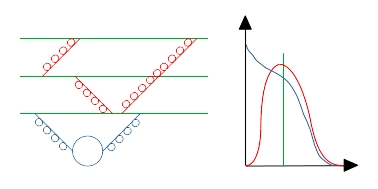
\includegraphics[width=0.8\linewidth]{DIS_nucleon_structuur_pdf/valance_quark_dist.jpg}
    \caption{Schematische voorstelling van de quark verdeling}%
    \label{fig:valance_quark_dist}
\end{figure}

Toen voor het eerst de structuur functies werden onderzocht werd de scaling violation waargenomen. Of je nu naar puntdeeltjes kijkt met een hoge resolutie of lage resolutie zou je geen verschil mogen zien maar we zien dat dit niet zo is. Door de kortere waarneming hebben de zee quarks de tijd niet gehad om uit te middelen. De kans om een valentiequark te vinden is steeds moeilijker met hogere energieën.

\begin{figure}[h]
    \centering
    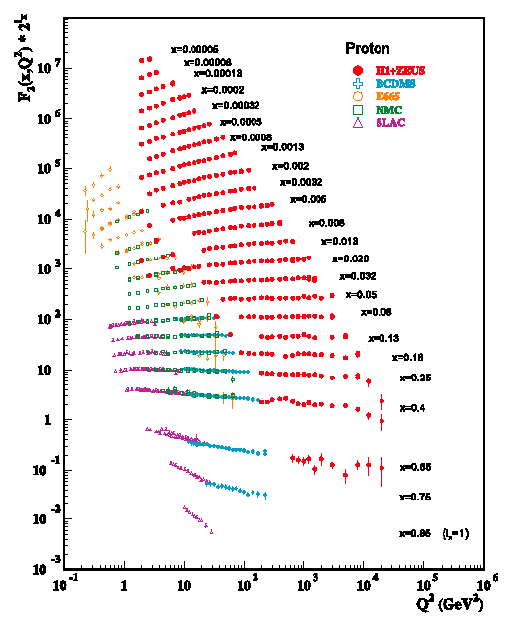
\includegraphics[width=0.4\linewidth]{DIS_nucleon_structuur_pdf/scale_viol.png}
    \caption{Scaling violations}%
    \label{fig:scale_viol}
\end{figure}

Het mooie is dat we met QCD e $Q^2$ afhankelijkheid kan beschrijven. Jammergenoeg kan dit niet gezegd worden over de $x$ afhankelijkheid. De scaling violation kan ook waargenomen worden. Uit  de structuur functies kunnen de parton distributie functies afgeleid worden. Hier zien we dat de zee quarks zullen domineren bij lagere $x$ waarden.

\begin{figure}[h]
    \centering
    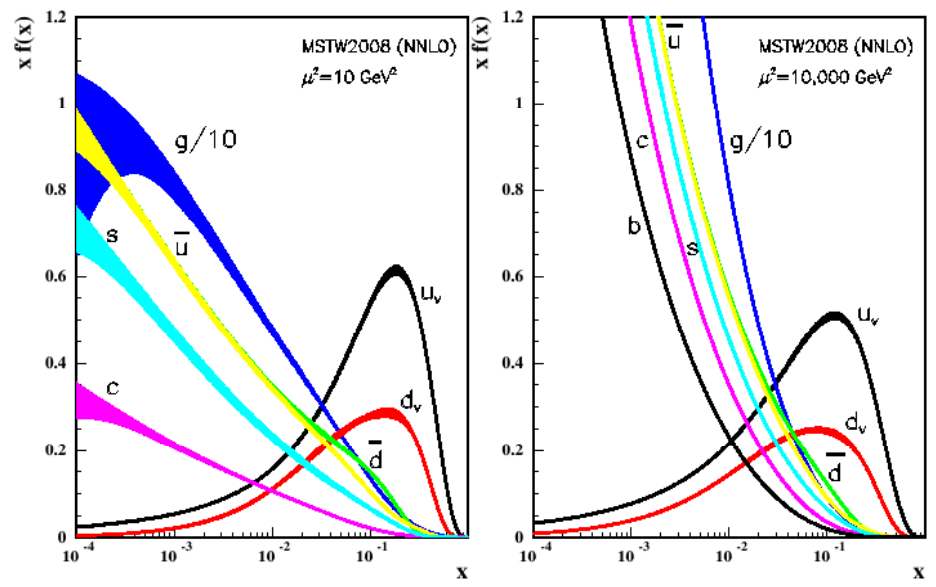
\includegraphics[width=0.6\linewidth]{DIS_nucleon_structuur_pdf/part_dist_func.png}
    \caption{parton distributie functies}%
    \label{fig:part_dist_func}
\end{figure}

We zien dat er voor hoge $x$ in het proton er meer $\overline d$ aanwezig is de $\overline u$. Dit is te verklaren door de pion wolk die rond het proton zal leven. Deze pionen kunnen alleen neutraal of positief geladen zijn wat zorgt voor die hogere densiteit aan $\overline d$. {\color{red} Dit durft hij graag vragen op het examen les 5 10u00}.

\subsection{Gepolariseerde DIS}%
\label{sub:gepolariseerde_dis}

Vanaf de jaren 80 zijn er ook longitudinaal gepolariseerde lepton en nucleon bundels gebruikt. Met deze experimenten kijken we naar de spin structuur van de nucleonen. We zien uit deze experimenten dat de spin van het proton niet zal opgemaakt zijn uit de valentie quarks. Dit leide tot de zo genoemde ``spin crisis''.

\subsection{Spin physics}%
\label{sub:spin_physics}

Als we kijken naar eender welk rond draaiend systeem zoals bijvoorbeeld het zonnestelsel, kunnen we zien dat het grootste deel van het angulaire momentum van deze systemen niet zal afhangen van de lichamen met de grootste massa.

\subsection{Nucleon spin fysica}%
\label{sub:nucleon_spin_fysica}

Uit de gepolariseerde experimenten verwachten we te zien dat $\frac{1}{2} = \frac{1}{2} (\Delta u + \Delta d)$ is. In het echt zien we dat de $\Delta u + \Delta d \approx 0$ wat natuurlijk totaal onverwacht was.\\
In de werkelijkheid is het veel veel complexer.
\begin{equation}
    \begin{aligned}
        \label{eq:spin_werkelijk}
        S_z &= \frac{1}{2} = \frac{1}{2} \Delta \Sigma + \Delta G + L_q + L_g\\
        \Delta \Sigma &= (\Delta u_v + \Delta d_v) + (\Delta u_s + \Delta d_s + \Delta \overline u+ \Delta \overline d+ \Delta \overline s)\\
        \Delta \Sigma &= \text{Quark spin contributie}\\
        \Delta G &= \text{Gluon spin contributie}\\
        L_q &= \text{Orbitaal angulair moment van quarks}\\
        L_g &= \text{Orbitaal angulair moment van gluons}\\
    \end{aligned}
\end{equation}
We verwachten wegens sferisch symmetrisch te zijn van de quarks dat al de bijdrages behalve $\Delta \Sigma$ 0 zouden zijn.\\

\begin{figure}[h]
    \centering
    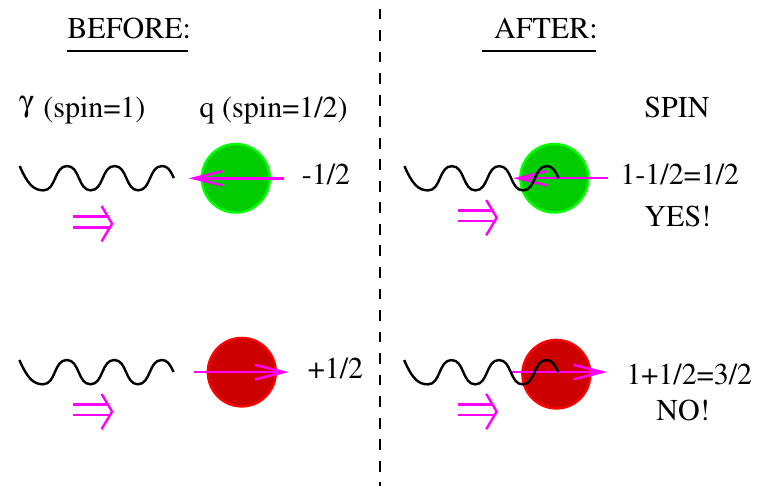
\includegraphics[width=0.8\linewidth]{DIS_nucleon_structuur_pdf/foton_abs_hel.png}
    \caption{Foton absorptie bij gepolariseerde DIS}%
    \label{fig:foton_abs_hel}
\end{figure}

Hoe meten we nu de spin distributie in quarks? We polariseren het proton parallel of anti parallel aan de richting van het foton en dan kijken we welke quarks het foton zullen absorberen. De reden waarom we het proton polariseren en niet de bundel is omdat het polariseren en vooral het flippen van de bundel die moeilijk is. Nu vragen we ons af het foton zal hitten. We kunnen ons de conservatie van heliciteit voorstellen bij absorptie. We zien in figuur \ref{fig:foton_abs_hel} dat de fotonen enkel geabsorbeerd worden door quarks met tegengestelde spin.\\
Steken we deze quarks nu in een nucleon en we nemen aan dat enkel de quarks contributies leveren aan de spin kunnen we door het verranderen van de polarisatie van het proton, kiezen we of we de quarks bekijken die ofwel positief of negatief bijdragen aan de spin van het proton. Door de onderste spin min de bovenste spin te doen in figuur \ref{fig:foton_abs_pol} dan krijgen we de netto bijdrage van de quarks aan de spin.

\begin{figure}[h]
    \centering
    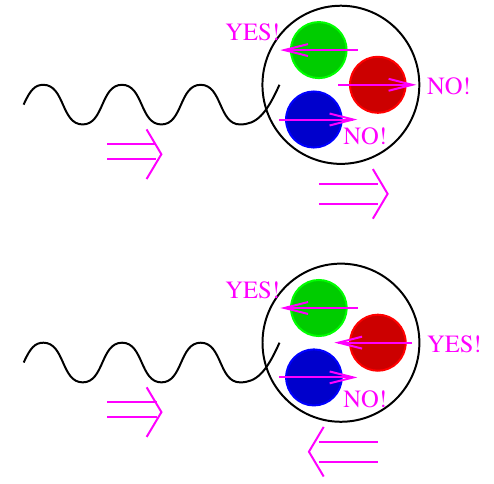
\includegraphics[width=0.6\linewidth]{DIS_nucleon_structuur_pdf/foton_abs_pol.png}
    \caption{Absorptie van foton door quarks in nucleon}%
    \label{fig:foton_abs_pol}
\end{figure}

Zo krijgen we uiteindelijk een tensor uit deze experimenten
\begin{equation}
    \begin{aligned}
        \label{eq:pol_tensor}
        W^{\mu\nu} = -g^{\mu\nu}&F_1(x,Q^2) + \frac{p^\mu p^\nu}{\nu} F_2(x,Q^2)\\
        &+ i\epsilon^{\mu\nu\delta\sigma} \frac{q_\delta}{\nu} (S_\sigma g_1(x,Q^2) + \frac{1}{\nu} (p\cdot qS_\sigma - S\cdot qp_\sigma)g_2(x,Q^2))
    \end{aligned}
\end{equation}
Hierbij kennen we de ongepolariseerde structuur functies $F_1$ en $F_2$ al. Dit komt neer op de impuls densiteit van de quarks:
\begin{equation}
    \begin{aligned}
        \label{eq:f_1_pol}
        F_1(x)=\frac{1}{2} \sum_q e_q^2[q^+(x)+q^-(x)] = \frac{1}{2} \sum_q e_q^2 q(x)
    \end{aligned}
\end{equation}

\begin{figure}[t!]
    \centering
    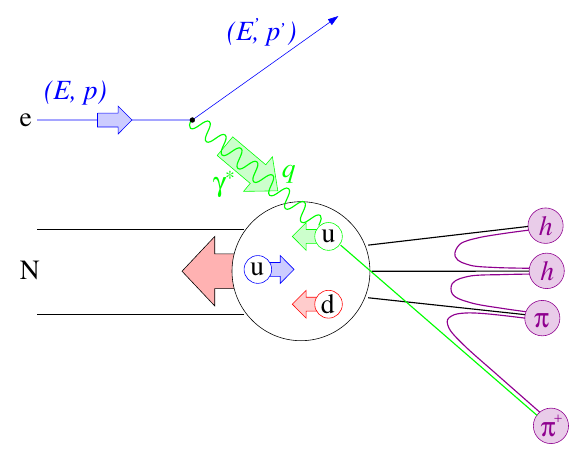
\includegraphics[width=0.6\linewidth]{DIS_nucleon_structuur_pdf/foton_abs.png}
    \caption{Onderzoek naar pin structuur}%
    \label{fig:foton_abs}
\end{figure}

De nieuwigheid hier is zijn de gepolariseerde structuur functies $g_1$ en $g_2$. Deze beschrijven de spin structuur van de spin van de quarks.
\begin{equation}
    \begin{aligned}
        \label{eq:g_1_pol}
        g_1(x)=\frac{1}{2} \sum_q e_q^2[q^+(x)-q^-(x)] = \frac{1}{2} \sum_q e_q^2 \Delta q(x)
    \end{aligned}
\end{equation}
$g_2$ zal niet besproken worden in deze cursus. Deze is te ingewikkeld. Hoe meten we $g_1$ nu. Het is natuurlijk niet mogelijk om het virtueel foton te polariseren. Wat wel mogelijk is, is het polariseren van de elektronbundel. Als de verstrooiing onder een grote hoek gebeurd nemen zal er een groot deel van de spin van het elektron overgebracht zijn naar het proton en als het onder een kleine hoek verstrooit wordt bijna geen spin overgebracht. Dit kan weergegeven worden in een polarisatie factor
\begin{equation}
    \begin{aligned}
        \label{eq:pol_factor}
        D= \frac{y(2-y)}{y^2 + 2(1-y)(1+R)}\\
        R= \frac{\sigma_L}{\sigma_T} 
    \end{aligned}
\end{equation}
Wat in deze experimenten zal gemeten worden is
\begin{equation}
    \begin{aligned}
        \label{eq:a_parallel}
        A_{||} &= \frac{\sigma^{\uparrow\downarrow} - \sigma^{\uparrow\uparrow}}{\sigma^{\uparrow\downarrow} + \sigma^{\uparrow\uparrow}}\\
               &= D.(A_1+\eta A_2)
    \end{aligned}
\end{equation}
Eigenlijk willen willen weten wat $A_1$ is
\begin{equation}
    \begin{aligned}
        \label{eq:a_parallel}
        A_{1} &= \frac{\sigma_{1/2} - \sigma_{3/2}}{\sigma^{1/2} + \sigma^{3/2}}\\
    \end{aligned}
\end{equation}
Zo bekomen we uiteindelijk een ratio
\begin{equation}
    \begin{aligned}
        \label{eq:pol_ratio_struct_func}
        \frac{g_1}{F_1} = \frac{1}{1+\gamma^2} \left( \frac{A_{||}}{D} - (\eta - \gamma)A_2\right)
    \end{aligned}
\end{equation}

De uiteindelijke structuur functies die we komen kan je vinden in figuur \ref{fig:pol_exp_res_1}. Voor het polariseren van het neutron maken we gebruik van $^3He$ als equivalent. We zien bij kleine $x$ niets wat wil zeggen dat de zee quarks niet toedragen tot de spin. Alle polarisatie is te vinden bij de hogere $x$ en zien we dat onze valentie quarks toch gepolariseerd zullen zijn. Bij het proton hebben we een positieve bijdrage en bij het neutron een negatieve bijdrage. Dit komt omdat de up quark positief zal bijdragen aan de spin en het down quark negatief. Het is momenteel nog niet gelukt om dit te bewijzen met QCD. In figuur \ref{fig:pol_exp_res_2} hebben we dit omgezet naar de bijdrages van de quarks zelf. Hieruit zien we dat de zee quarks niet gepolariseerd zijn. We krijgen uiteindelijk te zien dat $\Delta\Sigma \approx 0.30$ is, of anders gezegd dragen de spin van de quarks maar 1/3 mee aan de totale spin van het nucleon. Waar de rest vandaan komt is op dit moment nog niet duidelijk.

\begin{figure}[h]
    \centering
    \subfloat[]{
        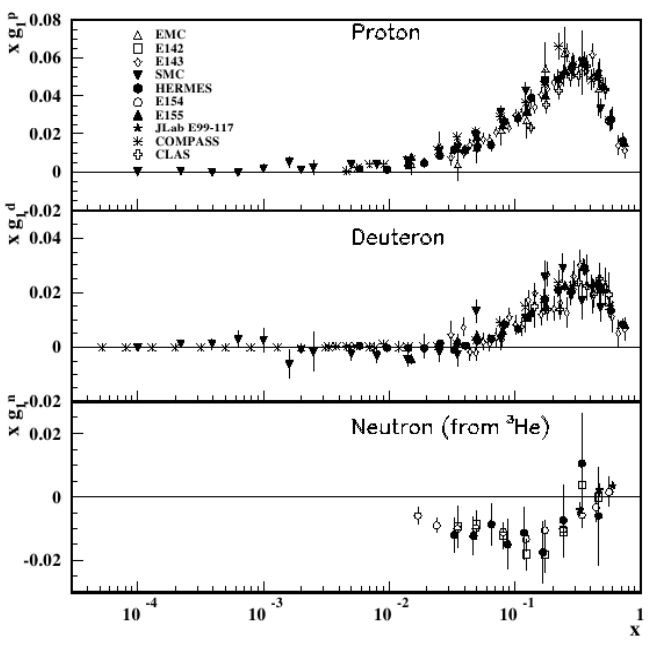
\includegraphics[width=0.5\textwidth]{DIS_nucleon_structuur_pdf/pol_exp_res_1.png}
        \label{fig:pol_exp_res_1}
    }
    \hfill
    \subfloat[]{
        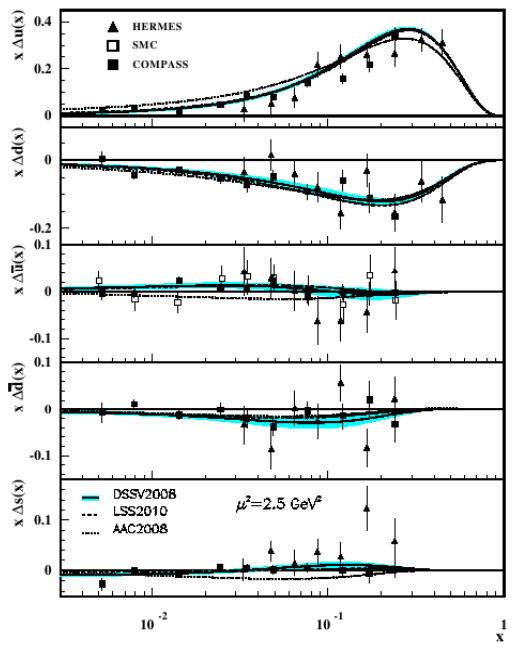
\includegraphics[width=0.4\textwidth]{DIS_nucleon_structuur_pdf/pol_exp_res_2.png}
        \label{fig:pol_exp_res_2}
    }
    \caption{Resultaten uit polarisatie experimenten}
\end{figure}

\subsection{Samenvatting van de structuur functies}%
\label{sub:samenvatting_van_de_structuur_functies}

Ten laatste voor dit hoofstuk kijken we nog eens naar een overzicht van wat we nu allemaal weten van de structuur functies.

\begin{figure}[h]
    \centering
    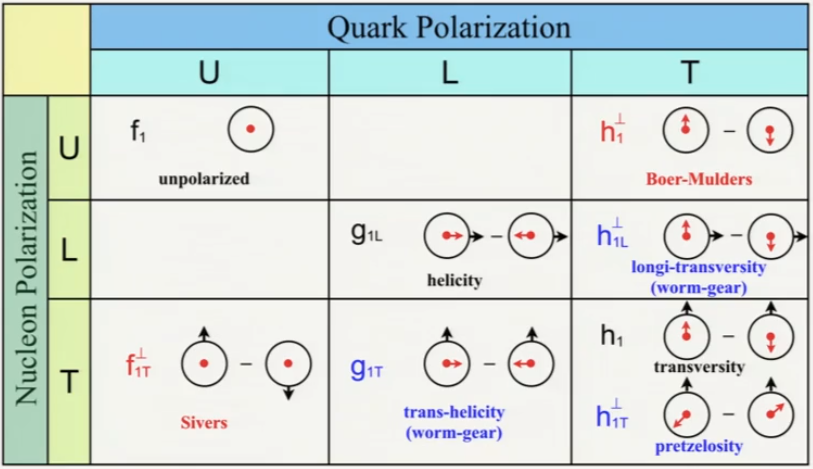
\includegraphics[width=0.8\linewidth]{DIS_nucleon_structuur_pdf/struct_func_samenvatting.png}
    \caption{Samenvatting van de structuur functies}%
    \label{fig:struct_func_samenvatting}
\end{figure}

\end{document}
